\documentclass{article}

\usepackage[utf8x]{inputenc}
\usepackage[T1]{fontenc}
\usepackage[francais]{babel}
\usepackage{xcolor}
\usepackage{listings}
\usepackage{mathptmx}
\usepackage{anyfontsize}
\usepackage{t1enc}
\usepackage[top=2cm, bottom=2cm, left=2cm, right=2cm]{geometry}
\usepackage{titlesec}
\usepackage{titling}
\usepackage{graphicx}
\usepackage[colorlinks = true,
            linkcolor = black,
            urlcolor  = black,
            citecolor = black,
            anchorcolor = black]{hyperref}

\newcommand{\changeurlcolor}[1]{\hypersetup{urlcolor=#1}}

\renewcommand\maketitlehooka{\null\mbox{}\vfill}
\renewcommand\maketitlehookd{\vfill\null}

\definecolor{codegreen}{rgb}{0,0.6,0}
\definecolor{codegray}{rgb}{0.5,0.5,0.5}
\definecolor{codepurple}{rgb}{0.58,0,0.82}
\definecolor{backcolour}{rgb}{0.95,0.95,0.92}
\definecolor{codekeywords}{rgb}{0.1,0.53,0.92}

\lstdefinestyle{c++}{
    backgroundcolor=\color{backcolour},   
    commentstyle=\color{codegreen},
    keywordstyle=\color{codekeywords},
    numberstyle=\tiny\color{codegray},
    stringstyle=\color{codepurple},
    basicstyle=\ttfamily\footnotesize,
    breakatwhitespace=false,         
    breaklines=true,                 
    captionpos=b,                    
    keepspaces=true,                 
    numbers=left,                    
    numbersep=5pt,                  
    showspaces=false,                
    showstringspaces=false,
    showtabs=false,                  
    tabsize=2,
    texcl=true,
    inputencoding=utf8,
    extendedchars=true,
    literate=
  {á}{{\'a}}1 {é}{{\'e}}1 {í}{{\'i}}1 {ó}{{\'o}}1 {ú}{{\'u}}1
  {Á}{{\'A}}1 {É}{{\'E}}1 {Í}{{\'I}}1 {Ó}{{\'O}}1 {Ú}{{\'U}}1
  {à}{{\`a}}1 {è}{{\`e}}1 {ì}{{\`i}}1 {ò}{{\`o}}1 {ù}{{\`u}}1
  {À}{{\`A}}1 {È}{{\'E}}1 {Ì}{{\`I}}1 {Ò}{{\`O}}1 {Ù}{{\`U}}1
  {ä}{{\"a}}1 {ë}{{\"e}}1 {ï}{{\"i}}1 {ö}{{\"o}}1 {ü}{{\"u}}1
  {Ä}{{\"A}}1 {Ë}{{\"E}}1 {Ï}{{\"I}}1 {Ö}{{\"O}}1 {Ü}{{\"U}}1
  {â}{{\^a}}1 {ê}{{\^e}}1 {î}{{\^i}}1 {ô}{{\^o}}1 {û}{{\^u}}1
  {Â}{{\^A}}1 {Ê}{{\^E}}1 {Î}{{\^I}}1 {Ô}{{\^O}}1 {Û}{{\^U}}1
  {œ}{{\oe}}1 {Œ}{{\OE}}1 {æ}{{\ae}}1 {Æ}{{\AE}}1 {ß}{{\ss}}1
  {ç}{{\c c}}1 {Ç}{{\c C}}1 {ø}{{\o}}1 {å}{{\r a}}1 {Å}{{\r A}}1
  {€}{{\EUR}}1 {£}{{\pounds}}1,
}
\lstset{style=c++}


\title{Simulation TP3\\Simulation de Monte Carlo et Intervalles de confiance}
\author{Arquillière Mathieu}
\date{\today}

\begin{document}

\begin{titlepage}
  \maketitle
\end{titlepage}

\tableofcontents
\newpage
\listoffigures
\newpage

\section{Introduction}
Dans ce TP, l'utilisation des nombres aléatoires est très importante. Sachant cela,
on ne se contentera pas de \emph{rand()} du C, on utilisera la bibliothèque de
M. Matsumoto découverte dans le TP précédent : \emph{Mersenne Twister}.

\section{Approximation de $\pi$ par la méthode de Monte Carlo}
\subsection{Méthode}
Ici la question est \emph{Comment approximer simplement le nombre $\pi$ grâce à des nombres aléatoires ?}
La méthode de Monte Carlo répond de la façon suivante :\\
Si on considère un cercle de centre $(0,0)$ et de rayon $r=1$, alors la surface
du quart supérieur droit (dans l'intervalle $[0;1],[0;1]$) de ce cercle est égale à $\frac{\pi}{4}$.
Puis si on réalise un certain nombre de tirages aléatoires de points $(x,y)$ avec $x,y \in [0;1]$,
alors le rapport du nombre de points à l'interieur du cercle sur le nombre total de points
se rapproche de la surface du quart du cercle.
$$
\frac{nombre\:de\:points\:dans\:le\:cercle}{nombre\:total\:de\:points} \approx \frac{\pi}{4}
\iff \pi \approx 4 \times \frac{nombre\:de\:points\:dans\:le\:cercle}{nombre\:total\:de\:points}
$$

\begin{figure}[!ht]
  \caption{Représentation graphique de la méthode Monte Carlo}
  \label{Méthode Monte Carlo}
  \centering
  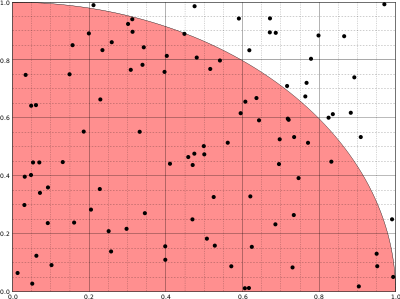
\includegraphics{images/monte_carlo_pi.png}
\end{figure}


\subsection{Code}
Une fois la méthode définie, la fonction d'approximation est très simple
à écrire. Il suffit de générer 2 nombres aléatoires dans l'intervalle $[0,1]$ représentant $x$ et $y$
puis tester si le point appartient au quart de cercle ($x\up{2} + y\up{2} < 1$).
Une particularité intéressante à noter est que pour faire ce simple calcul en C, on a plusieurs façons
de le faire et qui ne donnent pas exactement les même résultat. En effet pour faire le carré de $x$ et $y$
on peut utiliser la multiplication ($x \times x$) mais aussi la fonction \emph{pow} de \emph{math.h}.
Sur $1000000000$ d'itérations, il y a une différence à $10\up{-7}$ : $3.1415453920$ pour \emph{pow} contre
$3.1415455080$ pour la multiplication.
L'implémentation de cette fonction donne :

\begin{figure}[!ht]
\caption{Fonction d'approximation du nombre $\pi$ en utilisant la méthode de Monte Carlo}
\begin{lstlisting}[language=c++]
/**
* @brief Fonction permettant d'approximer le nombre PI
* 
* @param number Nombre d'itérations sur la méthode Monte-Carlo -> précision du retour
* @return double Approximation du nombre PI
*/
double approx_pi(int number)
{
    double x, y;
    int i, in = 0;

    // Monte-Carlo -> générer des points aléatoires entre 0 et 1 et faire le rapport de points
    // contenus dans le quart de cercle d'origine (0,0) et de rayon 1. Ce rapport est égal à PI/4
    for (i = 0; i < number; i++)
    {
        x = genrand_real1();
        y = genrand_real1();

        // Résultats differents en utilisant powf de <math.h>
        //if (pow(x, 2) + pow(y, 2) < 1)  // Resultat avec 1000000000 -> 3.1415453920
        if (x*x + y*y < 1)                // Resultat avec 1000000000 -> 3.1415455080
        {
            in++;
        }
    }
    return (double) in / (double)number * 4;
}
\end{lstlisting}
\end{figure}

\subsection{Résultats}

\subsubsection{1000000 itérations}
\begin{lstlisting}[language=c++]
  Approximation de PI:
  3.1447600000
\end{lstlisting}

\subsubsection{1000000000 itérations}
\begin{lstlisting}[language=c++]
  Approximation de PI:
  3.1415455080
\end{lstlisting}



\section{Expérimentations indépendantes}
\subsection{Principe}
L'objectif de cette partie est d'éxecuter un certain nombre de fois l'algorithme définit dans la
question précédente et d'obtenir plusieurs résultats afin d'observer la variance de l'algorithme.
Nous allons donc générer plusieurs approximations de $\pi$, les stocker dans un tableau et en
calculer la moyenne.

\subsection{Code}
Le code de cette fonction est très simple, on itere un certain nombre de fois (donné) et à chaque
itération on calcule une approximation de $\pi$ grâce à la fonction \emph{$approx\_pi()$} qu'on stocke
dans un tableau et qui incrémente une somme. Une fois fait, la fonction renvoie la moyenne calculée avec
la somme et le nombre d'itération.

\newpage
\begin{figure}
\caption{Fonction générant plusieurs approximations de $\pi$ et en calcule la moyenne}
\begin{lstlisting}[language=c++]
  /**
   * @brief Fonction utilisant plusieurs fois la fonction approx_pi() afin d'en faire une moyenne
   * 
   * @param[in] n nombre d'approximations de PI voulu
   * @param[out] pis tableau de taille @a n dans lequel on place les approximations de PI générées
   * @param[in] number nombre d'itérations pour générer chaque approximation avec la fonction approx_pi()
   * @return double moyenne des @a n approximations de PI
   */
  double mean_pi(int n, double* pis, int number)
  {
      int i;
      double sum = 0;
  
      // On fait plusieurs approximations de PI sans "redémarrer" le générateur de nombres aléatoires
      for (i = 0; i < n; i++)
      {
          pis[i] = approx_pi(number);
          sum += pis[i];
      }
      return sum / n;
  }
\end{lstlisting}
\end{figure}

\subsection{Résultats}

\subsubsection{100 approximations à 1000000 itérations}
\begin{lstlisting}[language=c++]
  Approximation de PI 100 x 1000000 fois:
3.1447600000 3.1398960000 3.1424280000 3.1422880000 3.1421200000 
3.1397280000 3.1398520000 3.1402960000 3.1393000000 3.1421880000 
3.1435480000 3.1422080000 3.1402320000 3.1389640000 3.1403880000 
3.1418800000 3.1424920000 3.1403960000 3.1407280000 3.1390400000 
3.1405520000 3.1449320000 3.1380960000 3.1429440000 3.1416320000 
3.1428920000 3.1407840000 3.1415320000 3.1383720000 3.1398040000 
3.1420440000 3.1438840000 3.1391920000 3.1421760000 3.1410240000 
3.1431880000 3.1393360000 3.1395560000 3.1402600000 3.1425240000 
3.1414760000 3.1416840000 3.1416520000 3.1424000000 3.1398760000 
3.1414840000 3.1371440000 3.1395360000 3.1378800000 3.1402800000 
3.1423280000 3.1409040000 3.1379760000 3.1397040000 3.1409960000 
3.1376920000 3.1427920000 3.1398840000 3.1423560000 3.1429040000 
3.1424440000 3.1439120000 3.1400280000 3.1395200000 3.1387560000 
3.1404160000 3.1405680000 3.1416320000 3.1444040000 3.1434880000 
3.1424880000 3.1405760000 3.1425840000 3.1429280000 3.1417360000 
3.1408880000 3.1404320000 3.1426320000 3.1420320000 3.1400080000 
3.1421840000 3.1403840000 3.1409800000 3.1427440000 3.1427360000 
3.1419000000 3.1416800000 3.1426640000 3.1421320000 3.1416720000 
3.1410760000 3.1416600000 3.1413120000 3.1427320000 3.1373680000 
3.1400640000 3.1417040000 3.1419040000 3.1438640000 3.1439000000

  Moyenne -> 3.1412453600
  M_PI    -> 3.141592653589793115997963468544185161590576171875
\end{lstlisting}

\subsubsection{100 approximations à 100000000 itérations}
\begin{lstlisting}[language=c++]
  Approximation de PI 100 x 100000000 fois:
3.1412453600 3.1418606400 3.1415495200 3.1415317200 3.1417336000 
3.1416126000 3.1415884000 3.1413548000 3.1412916800 3.1416867600 
3.1416500000 3.1416367600 3.1416785200 3.1416522400 3.1413547200 
3.1412954000 3.1414700800 3.1418641600 3.1415461600 3.1416512800 
3.1415327600 3.1415748800 3.1414050800 3.1414960800 3.1415069200 
3.1414344000 3.1416090800 3.1415152800 3.1418269200 3.1416315600 
3.1415834800 3.1416241200 3.1418688400 3.1415604000 3.1416593200 
3.1417215200 3.1413596400 3.1416708800 3.1412849600 3.1414950400 
3.1417837200 3.1415762800 3.1414292000 3.1413204000 3.1417708400 
3.1414347600 3.1411292000 3.1416093600 3.1414788800 3.1416279600 
3.1416208000 3.1413696400 3.1417154800 3.1413829200 3.1416954000 
3.1417977200 3.1413393200 3.1416194000 3.1413980000 3.1416571600 
3.1413948800 3.1413844400 3.1413628400 3.1415645200 3.1417590000 
3.1413988400 3.1415516000 3.1415472400 3.1416886000 3.1414753600 
3.1415731200 3.1417672000 3.1415502000 3.1415254800 3.1418243600 
3.1415437600 3.1418079200 3.1414720000 3.1415581600 3.1417345200 
3.1416936800 3.1415760400 3.1413869600 3.1414792800 3.1417000000 
3.1416924800 3.1417818800 3.1415389200 3.1414580400 3.1415749200 
3.1413760000 3.1412791600 3.1417450000 3.1416864400 3.1415733200 
3.1416333600 3.1416112000 3.1414257600 3.1416736800 3.1415289600 

  Moyenne -> 3.1415627112
  M_PI    -> 3.141592653589793115997963468544185161590576171875
\end{lstlisting}

\begin{figure}[!ht]
\caption{Sortie de \emph{gprof}, permettant d'observer le temps d'éxecution de chaque fonction}
\begin{lstlisting}[language=c++]
  Each sample counts as 0.01 seconds.
  %   cumulative   self              self     total           
 time   seconds   seconds    calls  ns/call  ns/call  name    
 27.83     36.55    36.55                             genrand_res53
 18.10     60.32    23.77 3020130816     7.87    11.58  approx_pi
 14.86     79.84    19.52                             confidences_intervals_95
 13.79     97.95    18.11                             genrand_real2
  8.78    109.48    11.53                             genrand_real3
  8.52    120.68    11.19 3020130816     3.71     3.71  genrand_int31
  5.08    127.35     6.67                             genrand_real1
  2.98    131.26     3.91                             genrand_int32
  0.18    131.49     0.23                             get_quantil
\end{lstlisting}
\end{figure}

\section{Intervalles de confiance}
\subsection{Principe}
L'objectif de cette partie est de déterminer des intervalles de confiance à 95\%
autour de la moyenne. Pour ça, on a besoin de calculer la variance :
$$
S^2(n) = \frac{\sum\limits_{n=1}^{n} (X_i - \overline{X}(n))^2}{n-1}
$$

Avec ce calcul on obtient le rayon de confiance :
$$
R = t_{n-1,1-\alpha/2} \times \sqrt{\frac{S^2(n)}{n}}
$$

où $t_{n-1,1-\alpha/2}$ est un quantil, récupéré dans le tableau suivant :\\\\
\begin{tabular}{|c|c|c|c|c|c|c|c|}
  \hline
  $1 \le n \le 10$ & $t_{n-1,1-\alpha/2}$ & $11 \le n \le 20$ & $t_{n-1,1-\alpha/2}$ & $21 \le n \le 30$ & $t_{n-1,1-\alpha/2}$ & $ n > 30$ & $t_{n-1,1-\alpha/2}$\\
  \hline
  1 & 12.706 & 11 & 2.201 & 21 & 2.080 & 40 & 2.021\\
2 & 4.303 & 12 & 2.179 & 22 & 2.074 & 80 & 2.000\\
3 & 3.182 & 13 & 2.160 & 23 & 2.069 & 120 & 1.980\\
4 & 2.776 & 14 & 2.145 & 24 & 2.064 & $\infty$ & 1.960\\
5 & 2.571 & 15 & 2.131 & 25 & 2.060 & &\\
6 & 2.447 & 16 & 2.120 & 26 & 2.056 & &\\
7 & 2.365 & 17 & 2.110 & 27 & 2.052 & &\\
8 & 2.308 & 18 & 2.101 & 28 & 2.048 & &\\
9 & 2.262 & 19 & 2.093 & 29 & 2.045 & &\\
10 & 2.228 & 20 & 2.086 & 30 & 2.042 & &\\
  \hline
\end{tabular}\\\\
Et ça nous donne l'intervalle de confiance :
$$
[\overline{X} - R, \overline{X} + R]
$$

\subsection{Code}
\subsubsection{Variance}
La première fonction à créer est celle qui calcule la variance. Elle a besoin de chaque
approximation de $\pi$ générée précédemment et de la moyenne correspondante. Ensuite
on exécute le calcul vu ci-dessus en calculant la somme avec une boucle.

\begin{figure}[!ht]
\caption{Fonction calculant la variance à partir d'un tableau d'approximation de $\pi$}
\begin{lstlisting}[language=c++]
/**
 * @brief Fonction calculant une estimation sans biais de la variance d'un tableau (en l'occurence de PI)
 * 
 * @param[in] n taille du tableau fourni
 * @param[in] pis tableau de taille @n contenant les approximations
 * @param[in] mean moyenne des approximations
 * @return double variance des approximations
 */
double variance(int n, double* pis, double mean)
{
    int i;
    double sum = 0;

    for (i = 0; i < n; i++)
    {
        sum += pow(pis[i] - mean, 2);
    }
    return sum / (n - 1);
}
\end{lstlisting}
\end{figure}

\subsubsection{Quantils}
Pour calculer le rayon de confiance $R$, on a besoin des qauntils. Pour modéliser
ceux-ci dans le code, on créer un tableau de correspondance avec tous les quantils
donnés dans le sujet.

\begin{figure}[!ht]
\caption{Implémentation des quantils - tableau}
\begin{lstlisting}[language=c++]
/**
 * @brief Tableau des quantiles
 */
const double t_values[] = {
    12.706, 4.303, 3.182, 2.776, 2.571, 2.447, 2.365, 2.308, 2.262, 2.228,
    2.201, 2.179, 2.160, 2.145, 2.131, 2.120, 2.110, 2.101, 2.093, 2.086,
    2.080, 2.074, 2.069, 2.064, 2.060, 2.056, 2.052, 2.048, 2.045, 2.042,
    2.021, 2.000, 1.980, 1.960
};
\end{lstlisting}
\end{figure}

Cependant ce sont les quantils pour $n \in [\![1;30]\!] \cap \{40, 80, 120, +\infty \}$
donc il faut également une fonction qui fasse correspondre $n$ avec les quantils.

\begin{figure}[!ht]
\caption{Implémentation des quantils - fonction de correspondance}
\begin{lstlisting}[language=c++]
/**
 * @brief Fonction qui permet d'obtenir les quantils à partir du tableau t_values
 * 
 * @param[in] ind indice du quantil voulu ([1, 30], 40, 80, 120, inf)
 * @return double quantil correspondant
 */
double get_quantil(int ind)
{
    int result = 0;
    if (ind <= 30)
        result = ind - 1;
    else if (ind == 40)
        result = 30;
    else if (ind == 80)
        result = 31;
    else if (ind == 120)
        result = 32;
    else
        result = 33;
    return t_values[result];
}
\end{lstlisting}
\end{figure}

\newpage
\subsubsection{Intervalle de confiance à 95\%}
Maintenant qu'on a la moyenne, la variance et les quantils, on peut créer la fonction
qui calcule l'intervalle de confiance à 95\% :

\begin{figure}[!ht]
\caption{Fonction calculant les intervalles de confiance à 95\%}
\begin{lstlisting}[language=c++]
/**
 * @brief Fonction qui calcule les intervalles de confiances à 95%
 * 
 * @param[in] n nombre d'occurences
 * @param[in] mean moyenne
 * @param[in] v variance
 * @param[out] b_inf borne inferieure de l'intervalle de confiance
 * @param[out] b_sup borne supérieur de l'intervalle de confiance
 */
void confidences_intervals_95(int n, double mean, double v, double * b_inf, double * b_sup)
{
    *b_inf = mean - get_quantil(n) * sqrt(v / n);
    *b_sup = mean + get_quantil(n) * sqrt(v / n);
}
\end{lstlisting}
\end{figure}

\subsection{Résultats}

\subsubsection{100 approximations à 1000000 itérations}

\begin{lstlisting}[language=c++]
Approximation de PI 100 x 1000000 fois:
  Moyenne -> 3.1412453600
  Variance -> 0.0000027833
  Intervalles de confiance: [3.1409183673, 3.1415723527]
\end{lstlisting}

\subsubsection{100 approximations à 100000000 itérations}

\begin{lstlisting}[language=c++]
Approximation de PI 100 x 100000000 fois:
  Moyenne -> 3.1415627112
  Variance -> 0.0000000243
  Intervalles de confiance: [3.1415321549, 3.1415932675]
\end{lstlisting}

\section{Simulation de population de lapin}
\subsection{Principe}
Ce problème est une façon d'aborder la suite de Fibonacci. En effet cette suite
reproduit le comportement de la population de lapins décrit dans le sujet :
2 lapins à l'initialisation, un couple se reproduit et donne 2 lapins à l'étape suivante.
Ceux-ci ne peuvent se reproduire qu'à l'étape d'après.
Ainsi, on peut connaître le nombre de lapins à l'étape $i$ en additionnant le nombre
de lapins à l'étape $i - 1$ et celui à l'étape $i - 2$.

\begin{figure}[!ht]
  \caption{Représentation de la suite de Fibonacci avec une population de lapins}
  \label{Suite de Fibonacci}
  \centering
  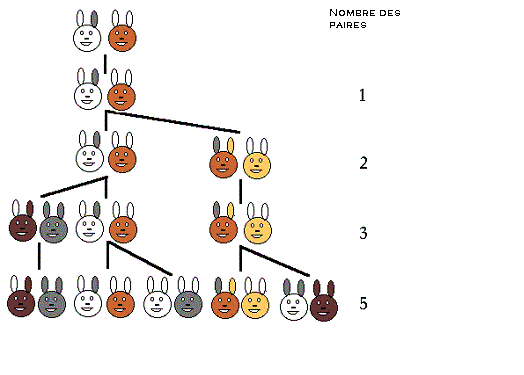
\includegraphics[scale=3]{images/lapins.png}
\end{figure}

\subsection{Code}
Cette suite se traduit simplement en code. On peut l'éxecuter de manière récursive
ou de manière itérative. Ici on a choisit de l'écrire de manière itérative.

\begin{figure}[!ht]
\caption{Fonction reproduisant la suite de fibonacci}
\begin{lstlisting}[language=c++]
  /**
  * @brief Fonction générant une population de lapins (Suite de Fibonacci)
  * 
  * @param[in] mois nombre de mois sur lesquels on observe l'évolution de la population de lapins
  * @param[in] long tableau de taille @a mois représentant le nombre de lapins chaque mois
  */
  void gen_lapins(int mois, unsigned long* population)
  {
      int i;
  
      population[0] = 1; // On démarre avec 1 couple au temps 0
      population[1] = 1; // Ce meme couple se retrouve au temps 1
  
      for (i = 2; i < mois; i++)
          population[i] = population[i - 1] + population[i - 2];
  }
\end{lstlisting}
\end{figure}

\subsection{Résultats}
Le tableau de population est un tableau de \emph{unsigned long} puisque les
nombres générés deviennent très grands très vite. En effet au delà de 90 mois, 
le nombre dépasse la taille de la variable et les résultats deviennent érronés.

\begin{figure}[!ht]
\caption{Affichage du tableau de population de couples de lapins}
\begin{lstlisting}[language=c++]  
Lapins: 
Mois  0:                    1  Mois  1:                    1  Mois  2:                    2  
Mois  3:                    3  Mois  4:                    5  Mois  5:                    8  
Mois  6:                   13  Mois  7:                   21  Mois  8:                   34  
Mois  9:                   55  Mois 10:                   89  Mois 11:                  144  
Mois 12:                  233  Mois 13:                  377  Mois 14:                  610  
Mois 15:                  987  Mois 16:                 1597  Mois 17:                 2584  
Mois 18:                 4181  Mois 19:                 6765  Mois 20:                10946  
Mois 21:                17711  Mois 22:                28657  Mois 23:                46368  
Mois 24:                75025  Mois 25:               121393  Mois 26:               196418  
Mois 27:               317811  Mois 28:               514229  Mois 29:               832040  
Mois 30:              1346269  Mois 31:              2178309  Mois 32:              3524578  
Mois 33:              5702887  Mois 34:              9227465  Mois 35:             14930352  
Mois 36:             24157817  Mois 37:             39088169  Mois 38:             63245986  
Mois 39:            102334155  Mois 40:            165580141  Mois 41:            267914296  
Mois 42:            433494437  Mois 43:            701408733  Mois 44:           1134903170  
Mois 45:           1836311903  Mois 46:           2971215073  Mois 47:           4807526976  
Mois 48:           7778742049  Mois 49:          12586269025  Mois 50:          20365011074  
Mois 51:          32951280099  Mois 52:          53316291173  Mois 53:          86267571272  
Mois 54:         139583862445  Mois 55:         225851433717  Mois 56:         365435296162  
Mois 57:         591286729879  Mois 58:         956722026041  Mois 59:        1548008755920  
Mois 60:        2504730781961  Mois 61:        4052739537881  Mois 62:        6557470319842  
Mois 63:       10610209857723  Mois 64:       17167680177565  Mois 65:       27777890035288  
Mois 66:       44945570212853  Mois 67:       72723460248141  Mois 68:      117669030460994  
Mois 69:      190392490709135  Mois 70:      308061521170129  Mois 71:      498454011879264  
Mois 72:      806515533049393  Mois 73:     1304969544928657  Mois 74:     2111485077978050  
Mois 75:     3416454622906707  Mois 76:     5527939700884757  Mois 77:     8944394323791464  
Mois 78:    14472334024676221  Mois 79:    23416728348467685  Mois 80:    37889062373143906  
Mois 81:    61305790721611591  Mois 82:    99194853094755497  Mois 83:   160500643816367088  
Mois 84:   259695496911122585  Mois 85:   420196140727489673  Mois 86:   679891637638612258  
Mois 87:  1100087778366101931  Mois 88:  1779979416004714189  Mois 89:  2880067194370816120  
Mois 90:  4660046610375530309  Mois 91:  7540113804746346429  Mois 92: 12200160415121876738  
Mois 93:  1293530146158671551  Mois 94: 13493690561280548289  Mois 95: 14787220707439219840  
Mois 96:  9834167195010216513  Mois 97:  6174643828739884737  Mois 98: 16008811023750101250  
Mois 99:  3736710778780434371    
\end{lstlisting}
\end{figure}

\newpage
\appendix
\section{Manuel d'utilisation}
La compilation du programme s'éxecute de la manière suivante grâce à \emph{gcc} :

\begin{lstlisting}[language=c++]
  gcc -o test.exe main.c mt19937ar.c -Wall -Wextra -O2 -lm
\end{lstlisting}
On a besoin de la librairie \emph{math.h} entre autre pour la fonction \emph{sqrt} 
et on utilise la génération de nombre aléatoire de \emph{M.Matsumoto} avec son code
contenu dans le fichier \emph{mt19937ar.c}.
On optimise le programme pour raccourcir les éxecutions des tests avec \emph{-O2}.

\section{Code}
\changeurlcolor{blue}\href{run:main.c}{Lien vers le code du main.c}

\section{Documentation}
\changeurlcolor{blue}\href{run:Documentation.pdf}{Lien vers la documentation Doxygen}

\end{document}
